\chapter{Multiscale turbulence measurements}
\label{ch:TurbulenceMeasurements}

\section{Experimental conditions}
\begin{figure}[h!]
  \centering
  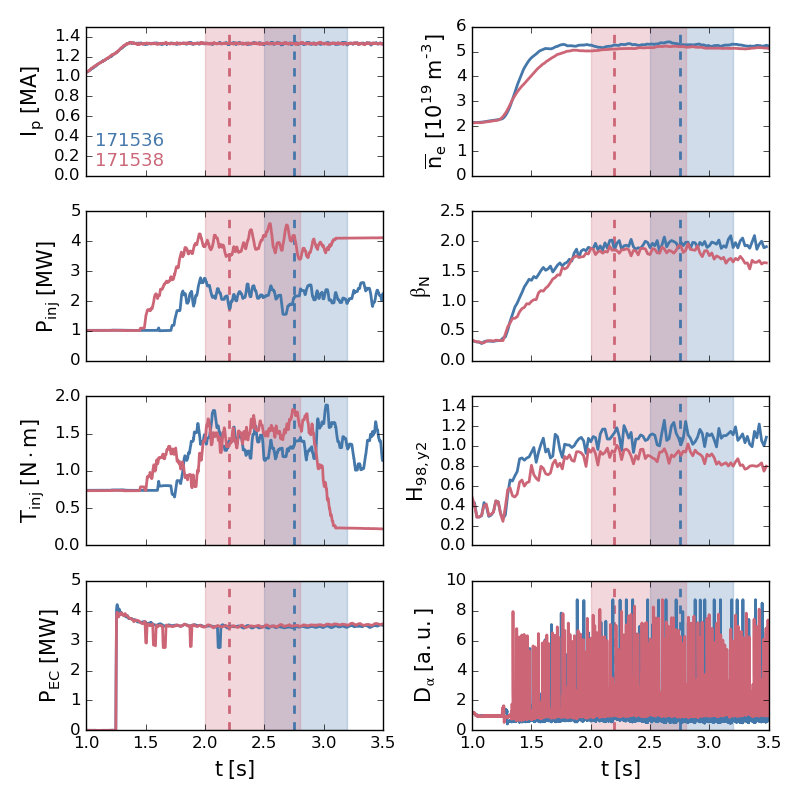
\includegraphics[width = \textwidth]{%
    Chapters/TurbulenceMeasurements/figs/traces.png}
  \caption[Plasma traces]{%
    Plasma traces.
  }
\label{fig:TurbulenceMeasurements:traces}
\end{figure}
\section{Measurements}
\begin{figure}[h!]
  \centering
  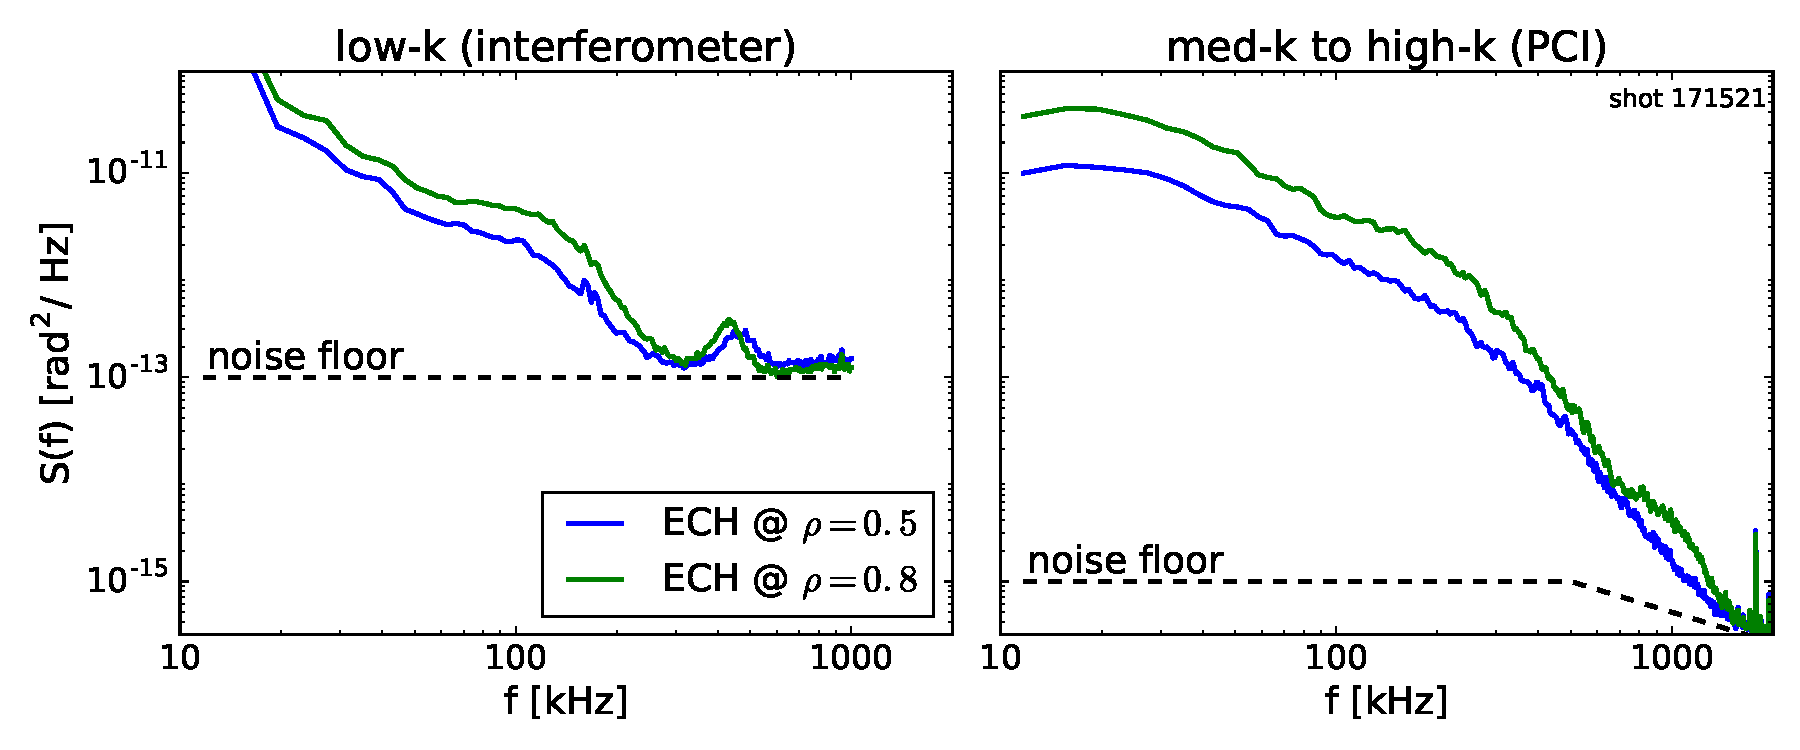
\includegraphics[width = 0.9 \textwidth]{%
    Chapters/TurbulenceMeasurements/figs/spectra_171521_quarterly_review.pdf}
  \caption[Combined PCI-interferometer measured spectra]{%
    Combined PCI-interferometer measured spectra.
  }
\label{fig:TurbulenceMeasurements:spectra_quarterly_review}
\end{figure}

\begin{figure}[h!]
  \centering
  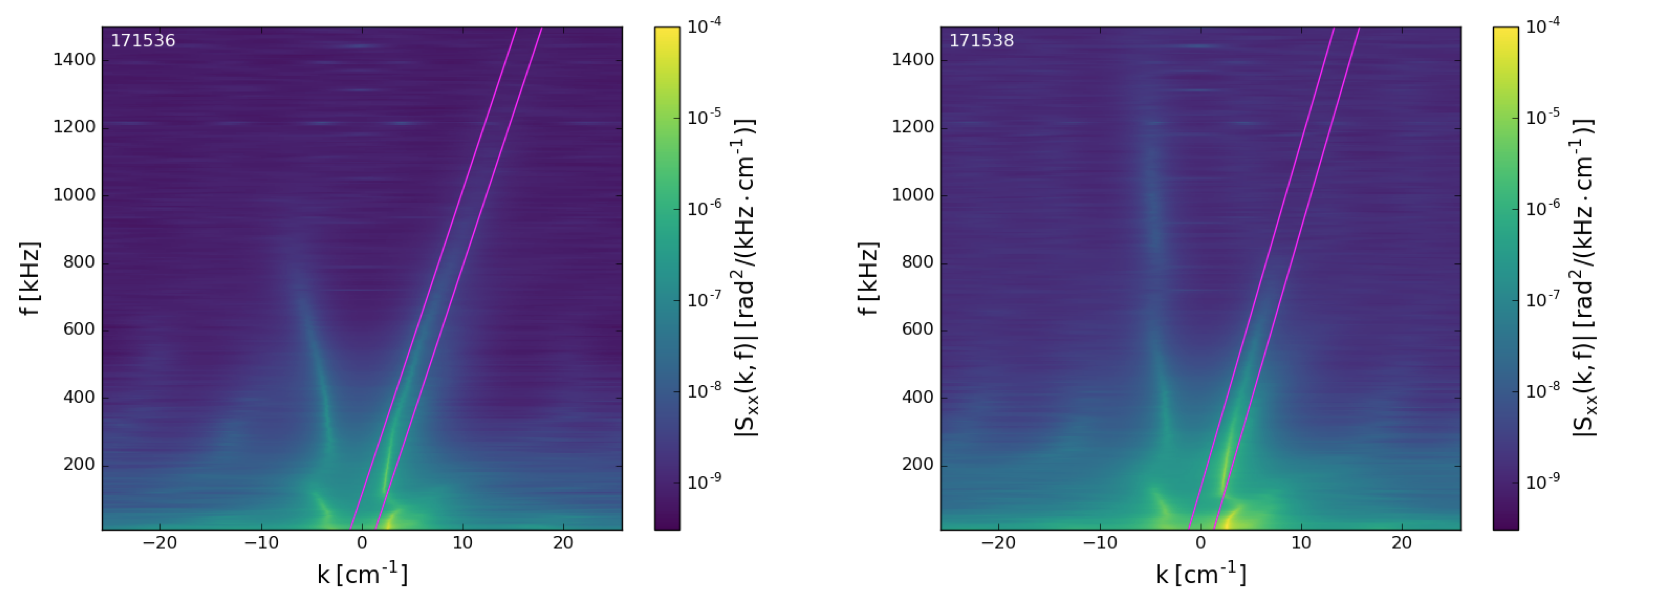
\includegraphics[width = \textwidth]{%
    Chapters/TurbulenceMeasurements/figs/Skf_annotated.png}
  \caption[PCI-measured $S(k, f)$ with branch annotations]{%
    PCI-measured $S(k, f)$ with branch annotations.
  }
\label{fig:TurbulenceMeasurements:Skf_annotated}
\end{figure}

\begin{figure}[h!]
  \centering
  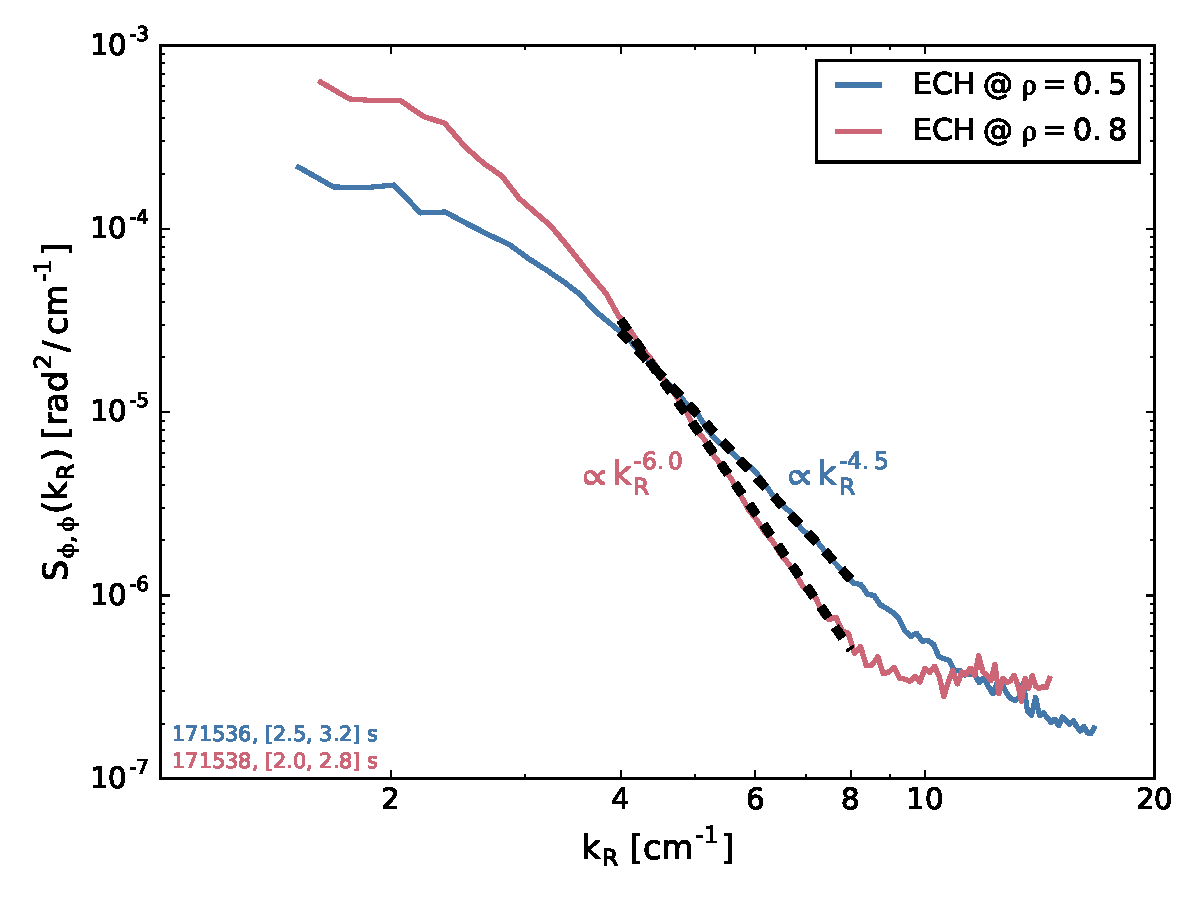
\includegraphics[width = 0.6 \textwidth]{%
    Chapters/TurbulenceMeasurements/figs/Sk_power_law.pdf}
  \caption[PCI-measured power law]{%
    PCI-measured power law from branches annotated in
    Figure~\ref{fig:TurbulenceMeasurements:Skf_annotated}.
  }
\label{fig:TurbulenceMeasurements:Sk_power_law}
\end{figure}


\section{TGLF modeling}
\begin{figure}[h!]
  \centering
  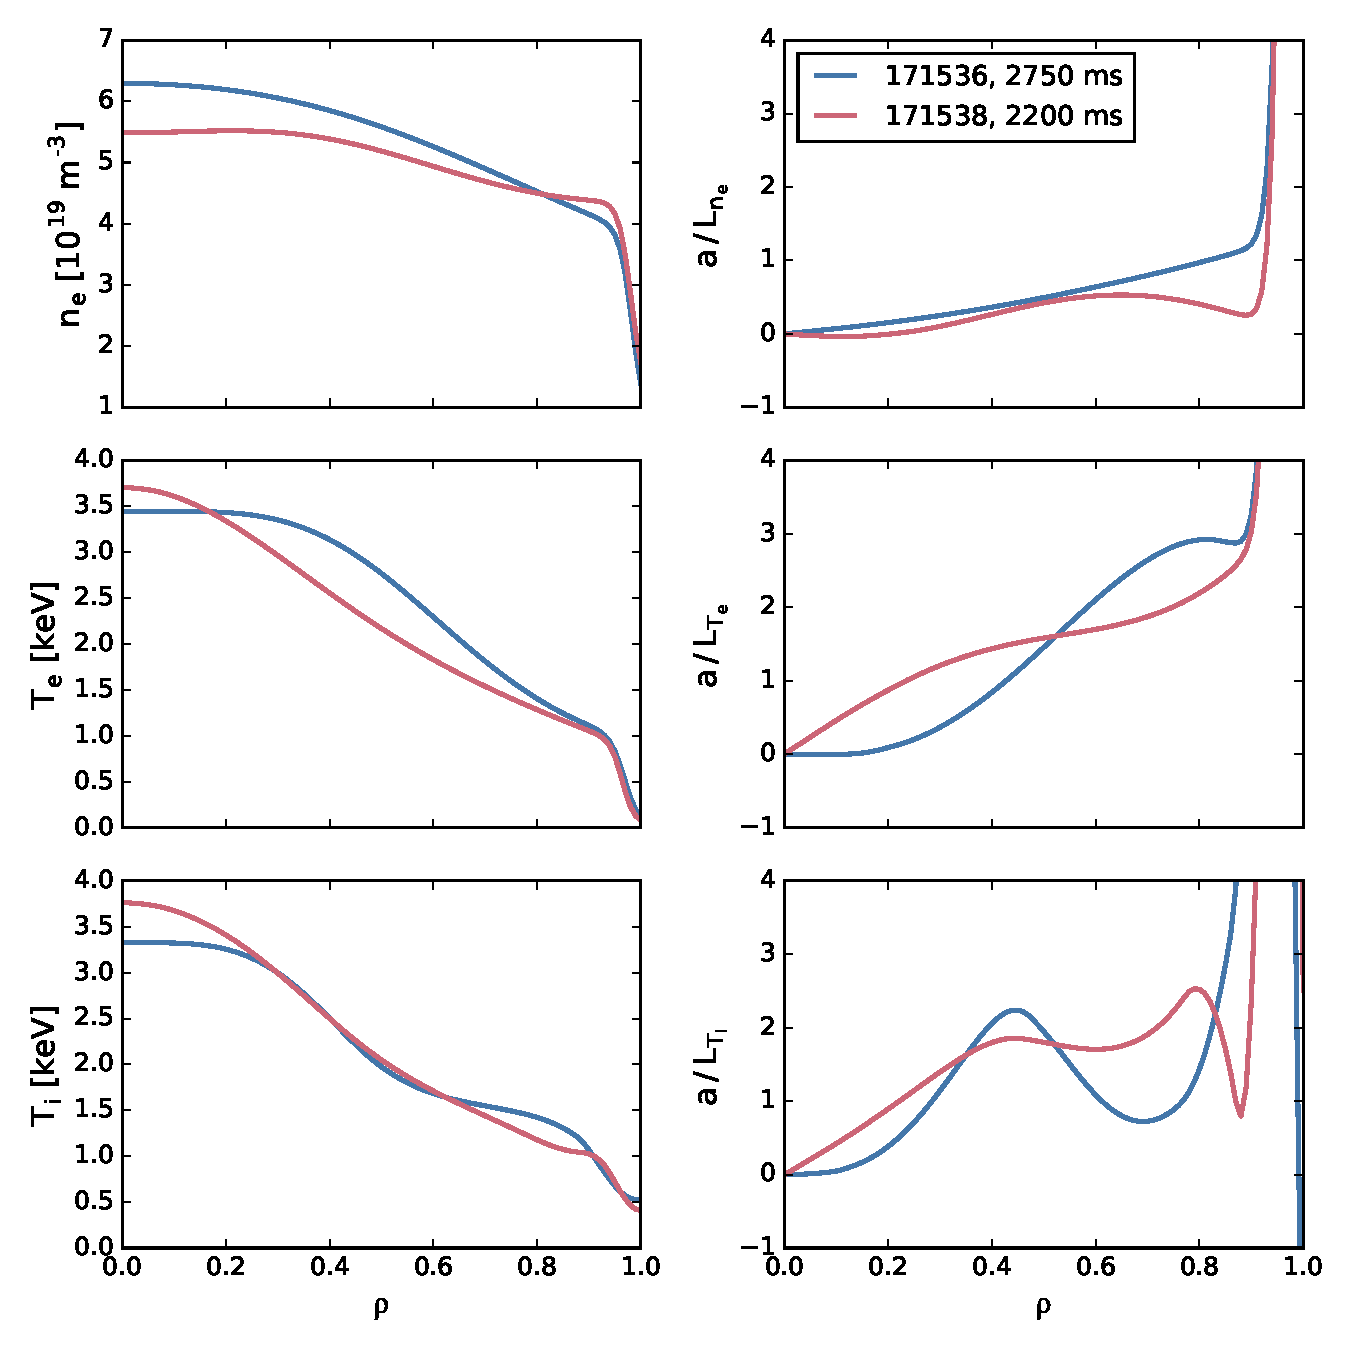
\includegraphics[width = \textwidth]{%
    Chapters/TurbulenceMeasurements/figs/profiles.pdf}
  \caption[Profiles \& inverse scale lengths]{%
    Profiles \& inverse scale lengths from
    OMFIT['TGLF\_scan']['tgyro\_output']
    used as input for TGLF simulations.
  }
\label{fig:TurbulenceMeasurements:profiles}
\end{figure}

\begin{figure}[h!]
  \centering
  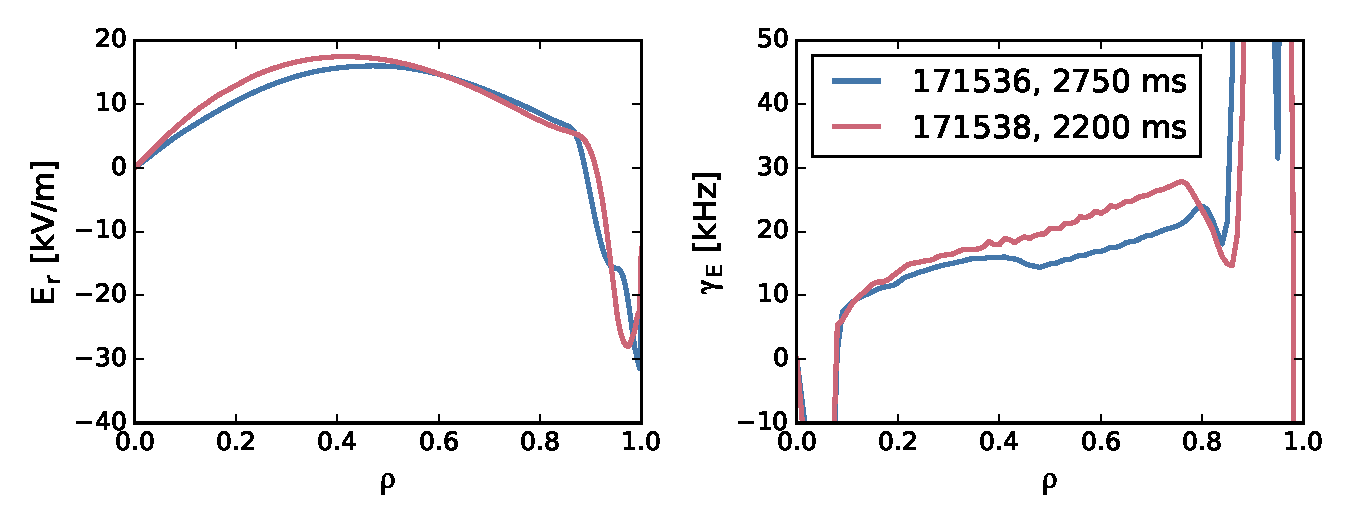
\includegraphics[width = \textwidth]{%
    Chapters/TurbulenceMeasurements/figs/Er_profiles.pdf}
  \caption[Radial electric field \& $E \times B$ shearing rate]{%
    Radial electric field \& $E \times B$ shearing rate from
    OMFIT['TGLF\_scan']['TGYRO']['PROFILES\_GEN']['OUTPUTS']['Er']
    (note that there are no corresponding values from
    OMFIT['TGLF\_scan']['tgyro\_output']
    from which Figure~\ref{fig:TurbulenceMeasurements:profiles}
    was generated, which is why this is a separate figure\ldots).
  }
\label{fig:TurbulenceMeasurements:Er_profiles}
\end{figure}

\begin{figure}[h!]
  \centering
  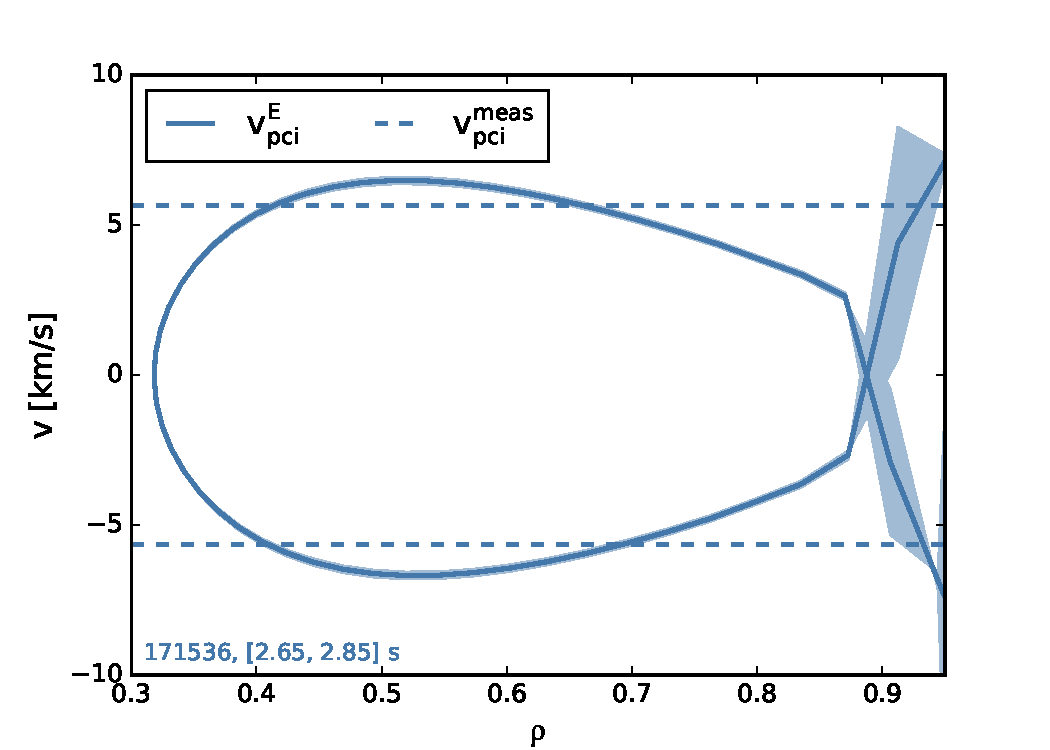
\includegraphics[width = \textwidth]{%
    Chapters/TurbulenceMeasurements/figs/doppler_shift.pdf}
  \caption[Doppler shift]{%
    Doppler shift. Positive \& negative values of $v_{\text{pci}}$
    correspond to above \& below the midplane, respectively.
    As the mask was not used, we cannot determine whether or not
    $v_{\text{meas}}$ corresponds to above or below the midplane, however
    (hence we plot $\pm v_{\text{meas}}$).
  }
\label{fig:TurbulenceMeasurements:doppler_shift}
\end{figure}

\begin{figure}[h!]
  \centering
  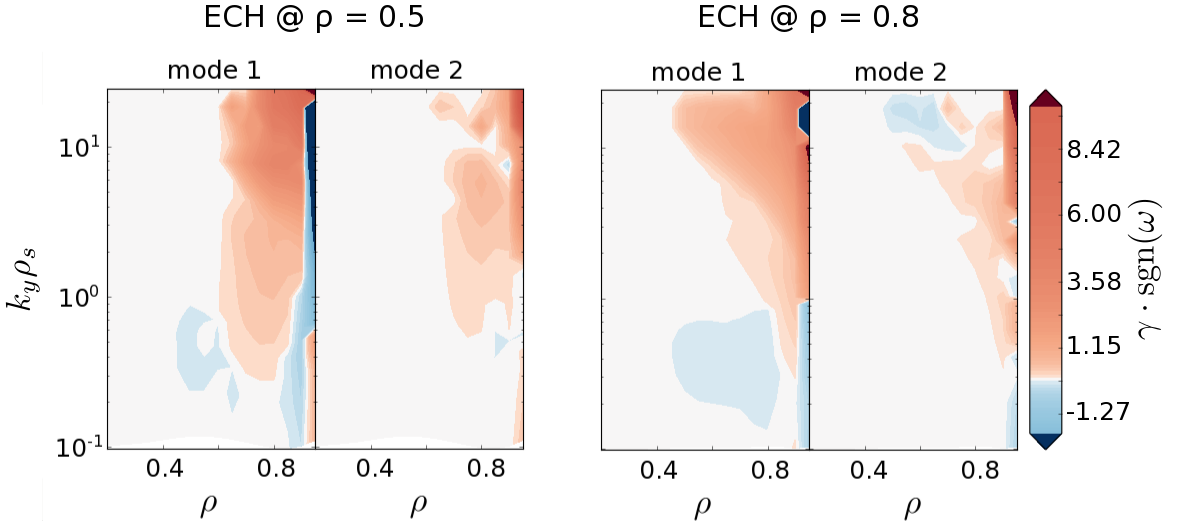
\includegraphics[width = \textwidth]{%
    Chapters/TurbulenceMeasurements/figs/TGLF_171536_vs_171538.png}
  \caption[Qualitative presentation of TGLF results]{%
    Qualitative presentation of TGLF results.
  }
\label{fig:TurbulenceMeasurements:TGLF_171536_vs_171538}
\end{figure}

\begin{figure}[h!]
  \centering
  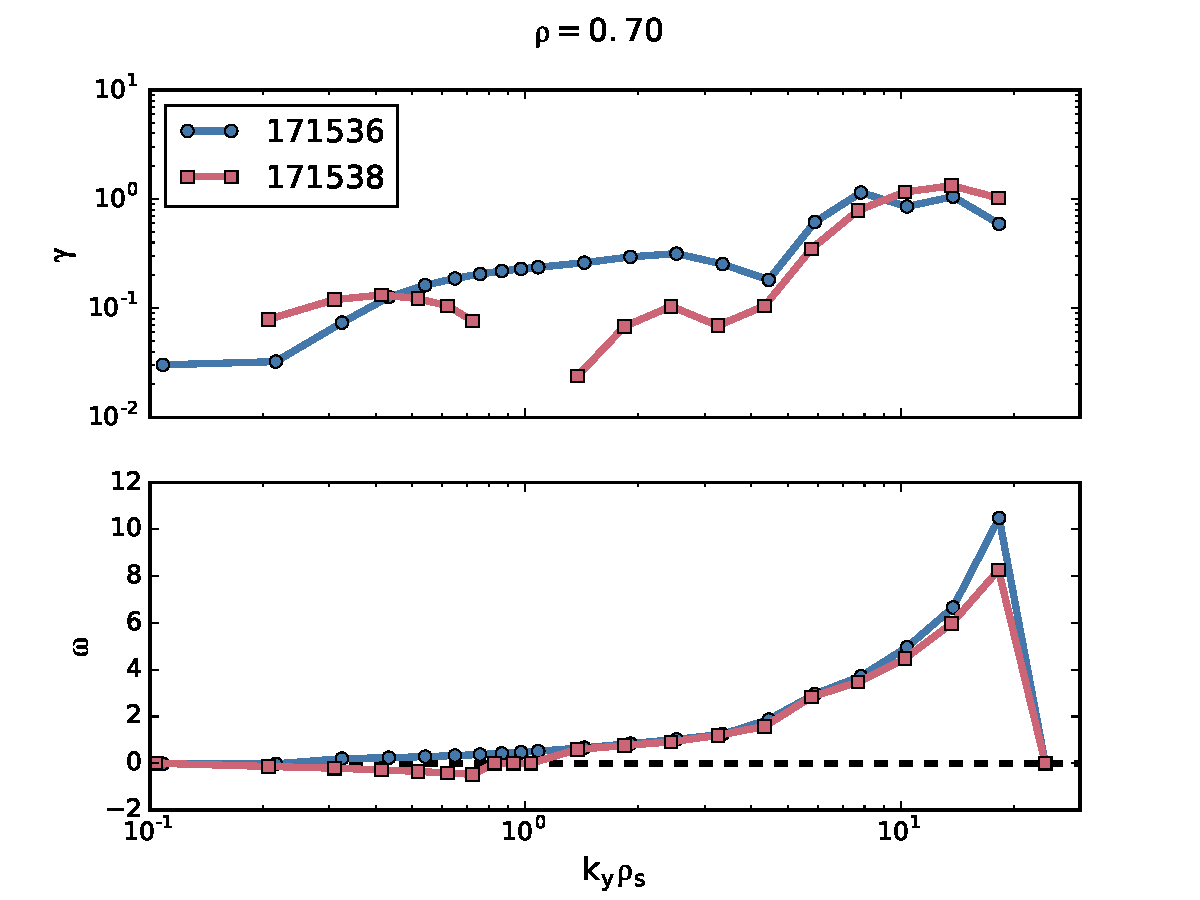
\includegraphics[width = \textwidth]{%
    Chapters/TurbulenceMeasurements/figs/linear_stability.pdf}
  \caption[Growth rates \& frequencies at $\rho=0.7$]{%
    Growth rates \& frequencies at $\rho=0.7$
    (i.e.\ we're slicing
    Figure~\ref{fig:TurbulenceMeasurements:TGLF_171536_vs_171538}
    at $\rho = 0.7$ for the most unstable mode, mode $1$).
    Note that only $171536$ uses SAT\_RULE $= 1$,
    which is calibrated against multiscale GYRO results;
    $171538$ uses SAT\_RULE $= 0$.
    Thus, it is difficult to draw conclusions\ldots
  }
\label{fig:TurbulenceMeasurements:linear_stability}
\end{figure}

\begin{figure}[h!]
  \centering
  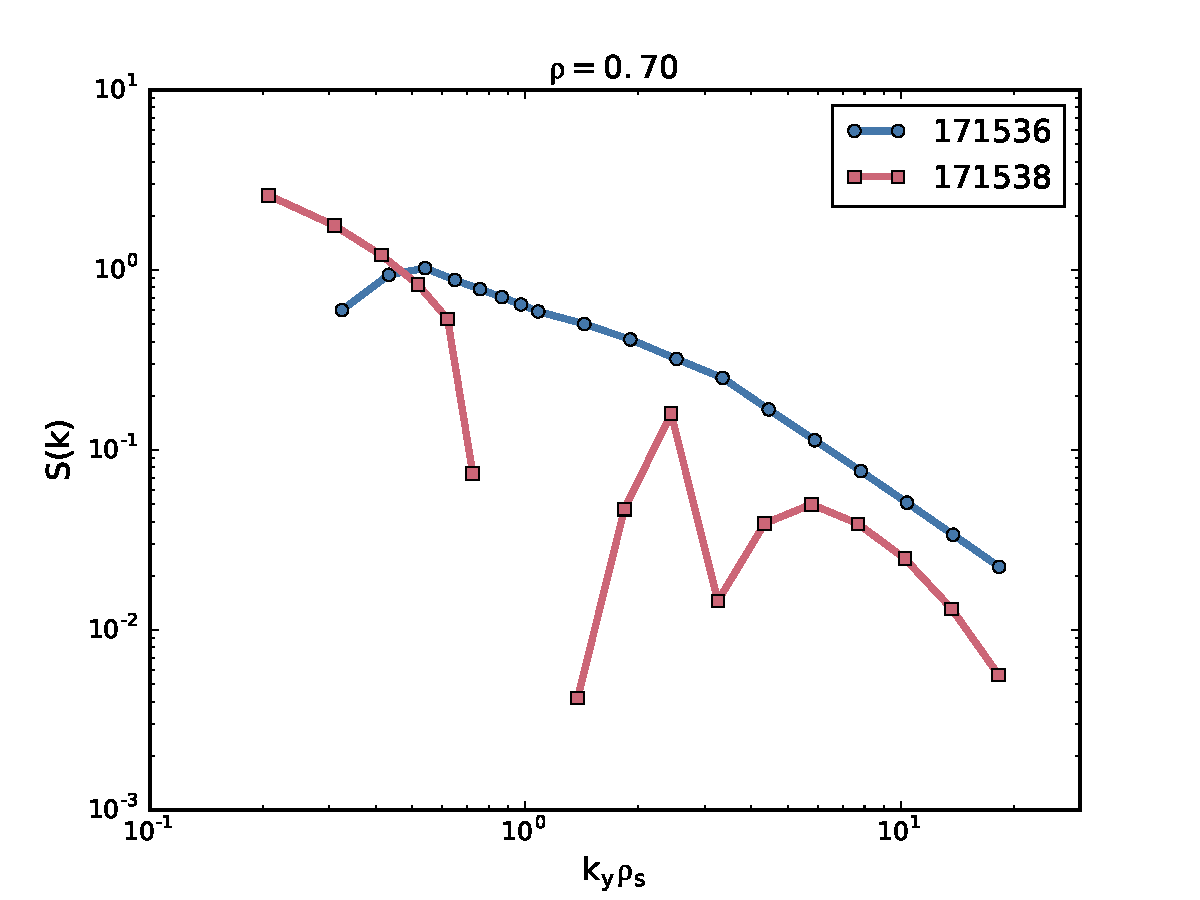
\includegraphics[width = \textwidth]{%
    Chapters/TurbulenceMeasurements/figs/density_spectra.pdf}
  \caption[TGLF-predicted density-fluctuation spectra at $\rho=0.7$]{%
    TGLF-predicted density-fluctuation spectra at $\rho=0.7$.
    Note that only $171536$ uses SAT\_RULE $= 1$,
    which is calibrated against multiscale GYRO results;
    $171538$ uses SAT\_RULE $= 0$.
    Thus, it is difficult to draw conclusions\ldots
  }
\label{fig:TurbulenceMeasurements:density_spectra}
\end{figure}
